\documentclass{standalone}
\usepackage{tikz}
\usetikzlibrary{arrows.meta}
\usepackage{amsmath}
\DeclareMathOperator{\Real}{Re}
\DeclareMathOperator{\Imag}{Im}
\begin{document}
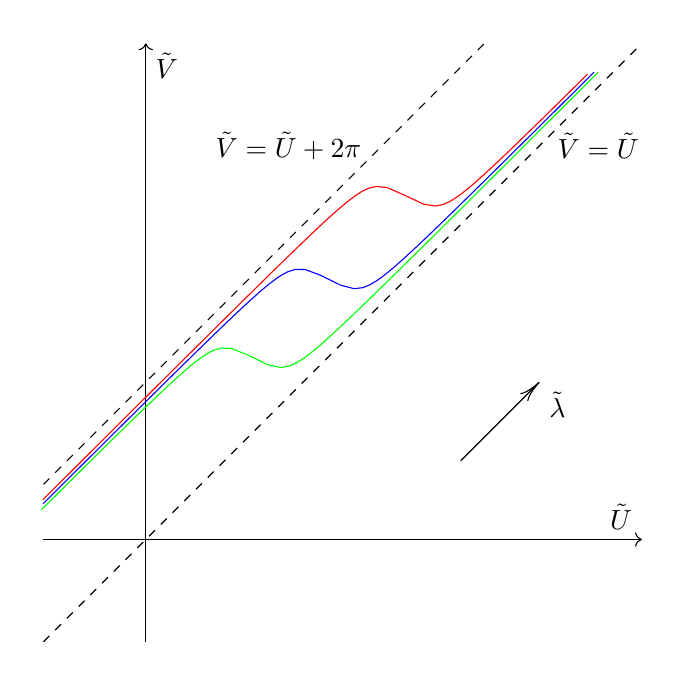
\begin{tikzpicture}
\clip (-1.5,-1.5) rectangle (6.5,6.5);

% \draw[color=gray,step=0.2,thin] (-10,-10) grid (10,10);
% \draw[color=darkgray,step=1.0,thick] (-10,-10) grid (10,10);

\draw[->] (-1.3,0)--(6.3,0) node[above left]{$\tilde{U}$};
\draw[->] (0,-1.3)--(0,6.3) node[below right]{$\tilde{V}$};

\draw[-{>[length=8pt,width=4pt]}] (4,1)--(5,2) node[below right]{$\tilde{\lambda}$};

\draw[dashed] (-1.3,-1.3) -- (5,5) node[right=3pt]{$\tilde{V} = \tilde{U}$} --(6.3,6.3);
\draw[dashed] (-1.3,0.7) -- (3,5) node[left=4pt]{$\tilde{V} = \tilde{U} + 2\pi$} --(4.3,6.3);

\draw[color=green,domain=0:8.2, samples=100] plot ({0.77*(\x + 2*atan(10*(\x-3))/360)-0.95}, {0.77*(\x - 2*atan(10*(\x-3))/360)});
\draw[color=blue,domain=-1.2:6.9, samples=100] plot ({0.77*(\x + 2*atan(10*(\x-3))/360)}, {0.77*(\x - 2*atan(10*(\x-3))/360)+1});
\draw[color=red,domain=-2.5:5.5, samples=100] plot ({0.77*(\x + 2*atan(10*(\x-3))/360)+1}, {0.77*(\x - 2*atan(10*(\x-3))/360)+2.05});

\end{tikzpicture}
\end{document}
